
% ----------------------------------------------------------------------
%  Set the document class
% ----------------------------------------------------------------------
\documentclass[11pt,a4paper,twoside]{article}

% ----------------------------------------------------------------------
% Define external packages, language, margins, fonts and new commands
% ----------------------------------------------------------------------
%\input{preamble} 
\usepackage[utf8]{inputenc}   % <<<<< Linux
\usepackage[english]{babel} % <<<<< English
\usepackage{notoccite}
\usepackage[skip=0.5\baselineskip]{caption}
\hyphenation{GTKWave}
\usepackage{listings}
\usepackage[all]{nowidow}

%blind text
\usepackage{lipsum}

\usepackage{graphicx}
\graphicspath{{./}{../../figlib/}{../mat/}{../sim/}}
\def\FontLn{% 16 pt normal
  \usefont{T1}{phv}{m}{n}\fontsize{16pt}{16pt}\selectfont}
\def\FontLb{% 16 pt bold
  \usefont{T1}{phv}{b}{n}\fontsize{16pt}{16pt}\selectfont}
\def\FontMn{% 14 pt normal
  \usefont{T1}{phv}{m}{n}\fontsize{14pt}{14pt}\selectfont}
\def\FontMb{% 14 pt bold
  \usefont{T1}{phv}{b}{n}\fontsize{14pt}{14pt}\selectfont}
\def\FontSn{% 12 pt normal
  \usefont{T1}{phv}{m}{n}\fontsize{12pt}{12pt}\selectfont}

% Use Arial font as default
%
\renewcommand{\rmdefault}{phv}
\renewcommand{\sfdefault}{phv}
\usepackage{geometry}	
\geometry{verbose,tmargin=2.5cm,bmargin=2.5cm,lmargin=2.5cm,rmargin=2.5cm}

%\usepackage{setspace}
%\renewcommand{\baselinestretch}{1.5}
\newcommand{\rvline}{\hspace*{-\arraycolsep}\vline\hspace*{-\arraycolsep}}

\usepackage[pdftex]{hyperref} % enhance documents that are to be
                              % output as HTML and PDF
\hypersetup{colorlinks,       % color text of links and anchors,
                              % eliminates borders around links
%            linkcolor=red,    % color for normal internal links
            linkcolor=black,  % color for normal internal links
            anchorcolor=black,% color for anchor text
%            citecolor=green,  % color for bibliographical citations
            citecolor=black,  % color for bibliographical citations
%            filecolor=magenta,% color for URLs which open local files
            filecolor=black,  % color for URLs which open local files
%            menucolor=red,    % color for Acrobat menu items
            menucolor=black,  % color for Acrobat menu items
%            pagecolor=red,    % color for links to other pages
            pagecolor=black,  % color for links to other pages
%            urlcolor=cyan,    % color for linked URLs
            urlcolor=black,   % color for linked URLs
	          bookmarks=true,         % create PDF bookmarks
	          bookmarksopen=false,    % don't expand bookmarks
	          bookmarksnumbered=true, % number bookmarks
	          pdftitle={report},
            pdfauthor={António Oliveira, 96512; Daniela Cardoso, 96517; Francisco Mendes, 96529},
%            pdfsubject={Thesis Title},
%            pdfkeywords={Thesis Keywords},
            pdfstartview=FitV,
            pdfdisplaydoctitle=true}

\usepackage[numbers,sort&compress]{natbib} % <<<<< References in numbered list [1],[2],...
\usepackage{subcaption} 
\usepackage{mdframed}
\usepackage{booktabs}
\usepackage{amsmath}
\usepackage{placeins}
\usepackage{amssymb}
\usepackage{epstopdf}


%%%%%%%% Resize equations
\usepackage{environ}         % provides \BODY
\usepackage{etoolbox}        % provides \ifdimcomp
\usepackage{adjustbox}       % provides \adjustbox
%% Resize equations
\newlength{\myl}
\let\origequation=\equation
\let\origendequation=\endequation
%% equationfit
\NewEnviron{equationfit}{
  \settowidth{\myl}{$\BODY$}                       % calculate width and save as \myl
  \origequation
  \ifdimcomp{\the\linewidth}{>}{\the\myl}
  {\ensuremath{\BODY}}                             % True
  {\resizebox{\linewidth}{!}{\ensuremath{\BODY}}}  % False
  \origendequation
}


%%%%%%%%%%%%%%%%%%%%%%%%%%%%%%%%%%%%%%%%%%%%%%%%%%%%%%%%%%%%%%%%%%%%%%%%
%     Begin Document                                                   %
%%%%%%%%%%%%%%%%%%%%%%%%%%%%%%%%%%%%%%%%%%%%%%%%%%%%%%%%%%%%%%%%%%%%%%%%


\usepackage{comment}

\begin{document}

% Set plain page style (no headers, footer with centered page number)
\pagestyle{plain}

% Set roman numbering (i,ii,...) before the start of chapters
%\pagenumbering{roman}

% ----------------------------------------------------------------------
%  Cover page
% ----------------------------------------------------------------------
%%%%%%%%%%%%%%%%%%%%%%%%%%%%%%%%%%%%%%%%%%%%%%%%%%%%%%%%%%%%%%%%%%%%%%%%
%                                                                      %
%     File: Thesis_FrontCover.tex                                      %
%     Tex Master: Thesis.tex                                           %
%                                                                      %
%     Author: Andre C. Marta                                           %
%     Last modified :  2 Jul 2015                                      %
%                                                                      %
%%%%%%%%%%%%%%%%%%%%%%%%%%%%%%%%%%%%%%%%%%%%%%%%%%%%%%%%%%%%%%%%%%%%%%%%

\thispagestyle {empty}

% IST Logo - Signature A
% parameters: bb=llx lly urx ury (bounding box), width=h_length, height=v_length, angle=angle, scale=factor, clip=true/false, draft=true/false. 
\includegraphics[bb=9.5cm 11cm 0cm 0cm,scale=0.29]{IST_A_CMYK_POS}

\begin{center}
%
% Figure (Image or plot)
\vspace{1.0cm}
% height = 50 mm
%\includegraphics[height=50mm]{Figures/Airbus_A350.jpg}

% Title, author and degree
\vspace{1cm}
{\FontLb Circuit Theory and Electronics Fundamentals} \\ % <<<<< EDIT TITLE
\vspace{1cm}
{\FontSn Department of Electrical and Computer Engineering, Técnico, University of Lisbon} \\ % <<<<< EDIT COURSE
\vspace{1cm}
{\FontSn T3 - AC/DC converter} \\
\vspace{1cm}
{\FontSn\it António Oliveira (96512), Daniela Cardoso (96517), Francisco Mendes (96529)} \\
\vspace{1cm}
{\FontSn May 8, 2021} \\ % <<<<< EDIT DATE (corresponds to date of oral examination)
%
\end{center}



% ----------------------------------------------------------------------
% Dedication page (optional)
% ----------------------------------------------------------------------
%\input{dedication} 
%\cleardoublepage

% ----------------------------------------------------------------------
%  Acknowledgments (optional)
% ----------------------------------------------------------------------
%\input{acknowledgements}
%\cleardoublepage

% ----------------------------------------------------------------------
%  Abstract (both in English and Portuguese)
% ----------------------------------------------------------------------
%\input{resumo} 
%\cleardoublepage

%\input{abstract} 

% ----------------------------------------------------------------------
%  Table of contents, list of tables, list of figures and nomenclature
% ----------------------------------------------------------------------

% Table of contents
%
\tableofcontents

% List of tables
%\addcontentsline{toc}{section}{\listtablename}
%\listoftables
%\cleardoublepage 

% List of figures
%\addcontentsline{toc}{section}{\listfigurename}
%\listoffigures
%\cleardoublepage 

% Set arabic numbering (1,2,...) after preface
%
%\setcounter{page}{1}
%\pagenumbering{arabic}

% ----------------------------------------------------------------------
%  Body
% ----------------------------------------------------------------------

\section{Introduction}
\label{sec:introduction}

% state the learning objective 
The purpose of this laboratory assignment is to make a Bandpass filter using OP-AMP, with the goal to get the highest merit, M, possible.
$$ M = \frac{1}{cost \times gainDeviation \times centralFreqDev}$$

Using the simplified circuit shown in Figure~\ref{fig:t5}, we tested different values for the resistors and capacitors and we found that the values in Table~\ref{tab:values} yielded the best merit. However, to get to those values, the real circuit in Figure~\ref{fig:t5-real} was used.

In Section~\ref{sec:simulation}, the circuit is analyzed by simulation using the software Ngspice. 

In Section~\ref{sec:analysis}, the circuit is analyzed theoretically using the software GNU Octave. 

In Section~\ref{sec:comparison}, a comparison is done between the results obtained by both analyses, theoretical and simulation, and a practical .

The conclusions of this study are outlined in Section~\ref{sec:conclusion}.

\begin{table}[ht!]
    \centering
    \begin{tabular}{c c}
    \toprule
    Component & Value \\ \midrule
    $C_1$  & 220 $nF$      \\
    $C_2$  & 110 $nF$      \\
    $R_1$  & 1 $k\Omega$   \\
    $R_2$  & 1 $k\Omega$   \\
    $R_3$  & 150 $k\Omega$ \\
    $R_4$  & 1 $k\Omega$   \\ \bottomrule
    \end{tabular}
    \caption{Resistance and Capacitance for the components}
    \label{tab:values}
\end{table}

\begin{figure}[ht!]
\centering
    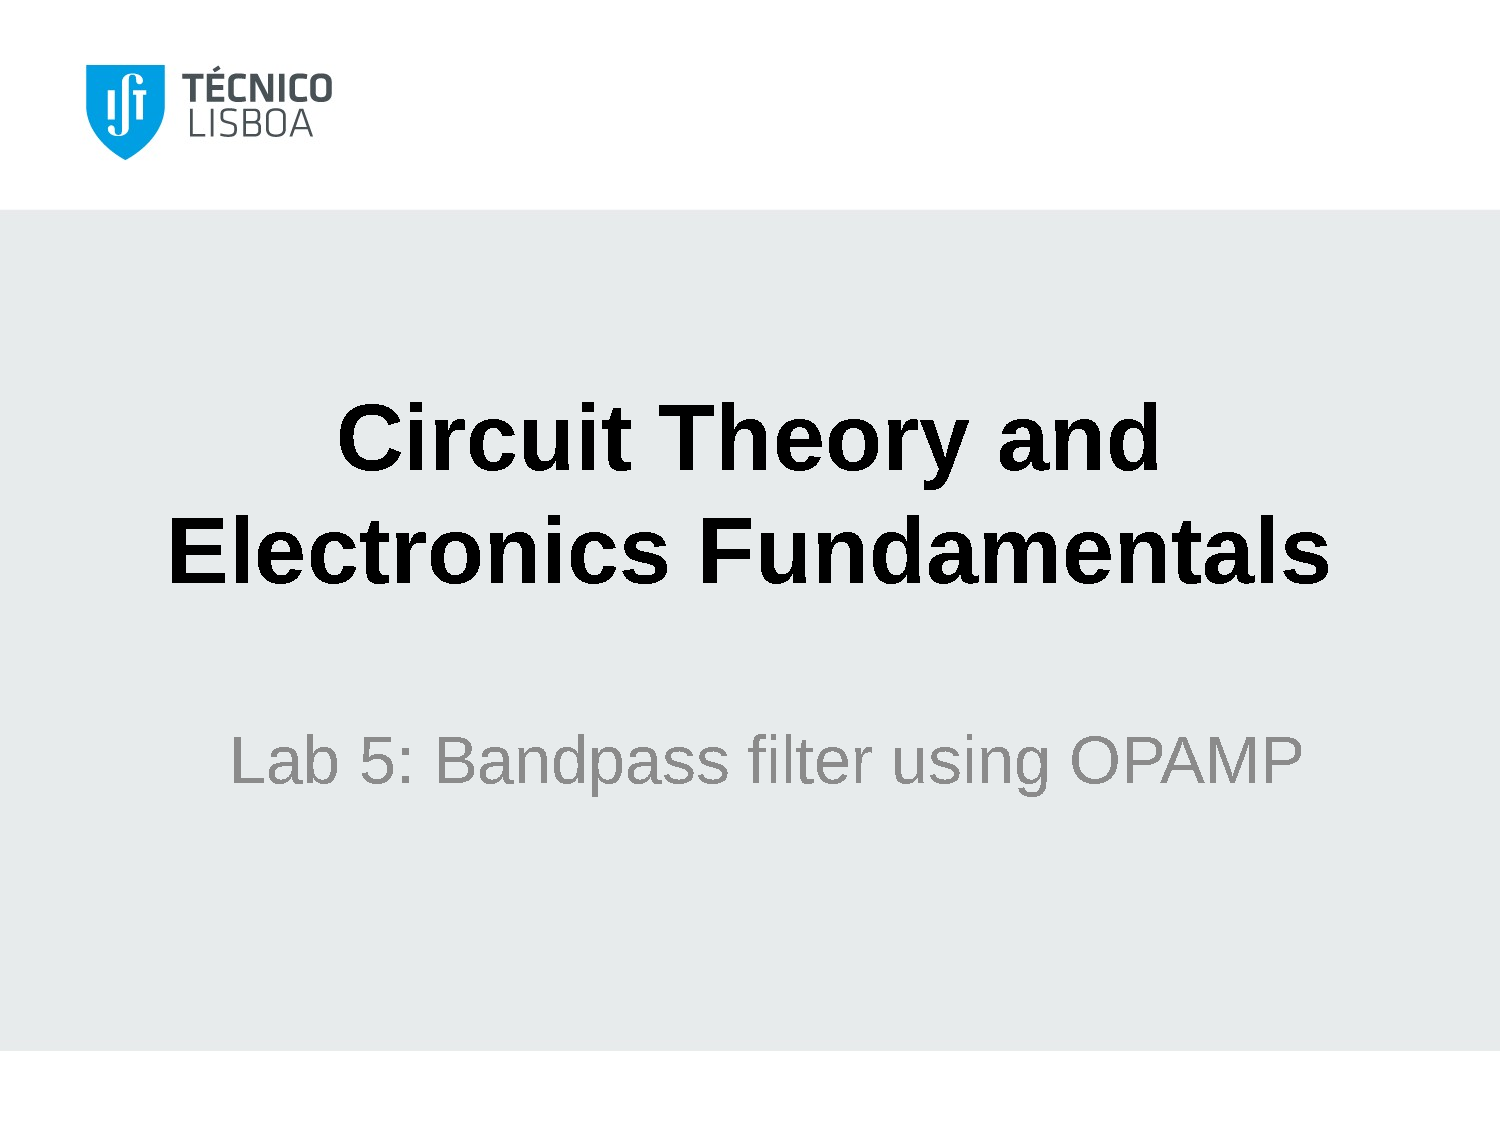
\includegraphics[width=0.8\linewidth]{t5.pdf}
\caption{Circuit T5, simplified.}
\label{fig:t5}
\end{figure}

\begin{figure}[ht!]
\centering
    \includegraphics[width=0.8\linewidth]{t5-real.pdf}
\caption{Circuit T5, real.}
\label{fig:t5-real}
\end{figure}

\FloatBarrier
\clearpage


%\clearpage
\section{Simulation Analysis}
\label{sec:simulation}


The plots obtained are shown in Figure~\ref{fig:votf}. The impedance at the input and
output, the gain, the lower and upper cut-off frequencies, the bandwidth, the cost and
the merit are presented in Table~\ref{tab:sim}.\\

\begin{minipage}[b]{0.49\textwidth}
  \centering
  \includegraphics[width=0.9\textwidth]{votf.pdf}
  \captionsetup{type=figure}
  \caption{Plots obtained by simulation.}
  \label{fig:votf}  
\end{minipage}
\hfill
\begin{minipage}[b]{0.49\textwidth}
  \centering
  \begin{tabular}{|c|c|}
      \hline
       & \textbf{Value} \\ \hline
      \input{../sim/inputZ_tab}
      \input{../sim/outputZ_tab}
      \input{../sim/merit_tab}
  \end{tabular}
  \captionsetup{type=table}
  \caption{Results obtained by simulation.}
  \label{tab:sim}
\end{minipage}


\section{Theoretical Analysis}
\label{sec:analysis}

In this section, the circuit is analyzed theoretically, according to the ideal
op-amp model ($Z_i =\infty$ and $Z_o=0$), resulting in the following equations:

\begin{gather}\label{step}
  |Z_i| = |Z_{C1} + R1 \parallelsum \infty| = |Z_{C1} + R1|\\
  |Z_o| = |Z_{C2} \parallelsum (R2 + R3 \parallelsum 0)| = |Z_{C2} \parallelsum R2|\\
  \begin{cases}
    v_- = v_+ = \frac{R1}{R1+Z_{C1}} v_i\\
    v_A = \left(1 + \frac{R3}{R4}\right) v_-\\
    v_o = \frac{Z_{C2}}{Z_{C2}+R2} v_A\\
  \end{cases}
\end{gather}

Solving the previous equations, the results are shown in Figure~\ref{fig:gain} and in Table~\ref{tab:NA}.\\

\begin{minipage}[b]{0.49\textwidth}
  \centering
  \includegraphics[width=0.9\textwidth]{gain.pdf}
  \captionsetup{type=figure}
  \caption{Plots obtained by theo. analysis.}
  \label{fig:gain}  
\end{minipage}
\hfill
\begin{minipage}[b]{0.49\textwidth}
  \centering
  \input{../mat/tabz}
  \captionsetup{type=table}
  \caption{Results obtained.}
  \label{tab:NA}
\end{minipage}




\section{Comparison}
\label{sec:comparison}

Comparing the results achieved in the simulation, Table~\ref{tab:t3}, and in the theoretical
analysis, Table~\ref{tab:vout}, it is possible to see a small difference.

This discrepancy may have resulted from the assumption made in Step~\ref{subsec:step1},
since $Ripple\ (\%)$ theoretical $\approx rippleperc$ simulated, and
$Deviation\ (\%)$ theoretical $\not\approx rippleperc$ simulated. 
However this assumption is needed, since without it, the analysis would become very difficult.

Additionally, there would be always some very small differences due to the non-linearity of the equations.


\section{Conclusion}
\label{sec:conclusion}

In this laboratory assignment, the objective of making a Bandpass filter using OP-AMP shown in
Figure~\ref{fig:t5-real} has been achieved.
The values for the components in Table~\ref{tab:values} has a merit of approximately $3,88 \times 10^{-6}$
and a cost of 13626,95 MU, with a gain of 39,98 dB and a central frequency of 981,37 $Hz$.

%\cleardoublepage

%\input{experiencia}
% ----------------------------------------------------------------------
%  Bibliography
% ----------------------------------------------------------------------
%\addcontentsline{toc}{section}{\bibname}
%\bibliographystyle{abbrvunsrtnat} % <<<<< SELECT IF USING REFERENCES BY NUMBER (CITATION ORDER)
%\bibliography{../../../BIBfile.bib}

% ----------------------------------------------------------------------
\end{document}
% ----------------------------------------------------------------------
